\documentclass[11pt]{article}
\usepackage[margin=1in]{geometry}
\usepackage[T1]{fontenc}
\usepackage{lmodern}
\usepackage{amsmath,amssymb}
\usepackage{graphicx}
\usepackage{array,tabularx}
\usepackage{tikz}
\usetikzlibrary{arrows.meta,positioning,fit,backgrounds}
\usepackage[hidelinks]{hyperref}
\usepackage{microtype}

\title{CSC490 Assignment 3: Pre-training Nanochat}
\author{Team member names and student IDs: \textit{to be added}}
\date{November 2026}

\begin{document}
\maketitle

\section{Architecture Review}
\subsection{What is nanochat?}
Nanochat is Andrej Karpathy's compact, end-to-end codebase for training and
serving a conversational language model. Its scope extends beyond the neural
network: it includes tokenization, pre-training, subsequent training stages,
evaluation, inference, and a chat interface~\cite{nanochat-readme}.
The underlying language model is a decoder-only Transformer that predicts
the next token from the preceding tokens. A causal attention mask prevents
each position from accessing future tokens. Pre-training learns this
next-token distribution; conversational behaviour also depends on subsequent
training and the data used, rather than on a separate ``chat'' layer.

\paragraph{Version scope.}
This architecture review and Figure~\ref{fig:original} describe the original
October 13, 2025 implementation, commit \texttt{3a5e0bc}, as requested in
Part One~\cite{nanochat-code}. The exploratory pilot below uses a separate
snapshot, commit \texttt{92d63d4} (July 3, 2026), as its July baseline.
The October architecture review and July experimental baseline describe
different snapshots and must not be treated as the same architecture.

\subsection{Original model architecture}
Given token IDs $t_1,\ldots,t_T$, a learned embedding matrix maps each token
to a vector of width $d$. Parameter-free root-mean-square normalization
(RMSNorm) is applied immediately after embedding. The sequence then passes
through $L$ Transformer blocks, followed by a final RMSNorm and a learned
output projection to vocabulary logits~\cite{nanochat-code}.

Each block has two pre-normalized residual sublayers. For residual-stream
input $X$, the block computes
\begin{align}
 U &= X + \operatorname{Attention}(\operatorname{RMSNorm}(X)),\\
 Y &= U + \operatorname{MLP}(\operatorname{RMSNorm}(U)).
\end{align}
The skip connections preserve a direct path through the block, while
normalization controls the scale of the inputs to each sublayer. In this
implementation, RMSNorm has no learned scale or bias, and the linear
projections are also bias-free.

\paragraph{Causal self-attention.}
Separate linear projections produce queries $Q$, keys $K$, and values $V$.
Rotary position embeddings (RoPE) are applied to $Q$ and $K$, followed by
per-head RMSNorm of both. Thus, the absence of an additive position-embedding
table does \emph{not} mean the model lacks positional information. With
processed queries and keys denoted $\widehat Q$ and $\widehat K$, each head
computes
\begin{equation}
 A = \operatorname{softmax}\!\left(
 \frac{\widehat Q\widehat K^{\mathsf T}}{\sqrt{d_h}}+M
 \right)V,
\end{equation}
where $d_h$ is the head dimension and $M$ masks future positions. The heads
are concatenated and projected back to width $d$. Every original block
uses full causal attention within the available context, not alternating
sliding-window and full-attention layers. The code supports fewer key/value
heads than query heads (grouped-query or multi-query attention), although
the original default uses equal head counts~\cite{nanochat-code}.

\paragraph{Feed-forward network.}
The MLP expands each position's representation from $d$ to $4d$, applies
squared ReLU, and projects back to $d$:
\begin{equation}
 \operatorname{MLP}(H)
 = \bigl[\operatorname{ReLU}(H W_1)\bigr]^{\odot 2}W_2,
 \qquad W_1\in\mathbb{R}^{d\times4d},\quad
 W_2\in\mathbb{R}^{4d\times d}.
\end{equation}
The square is elementwise. This is not a gated MLP such as SwiGLU.

\paragraph{Output and learning objective.}
The output projection is \emph{untied}: it does not share weights with the
input embedding matrix. Before computing the training loss or returning
inference logits, the model applies the soft cap
$\widetilde z=15\tanh(z/15)$. Training uses cross-entropy with next-token
targets. During generation, the logits determine the next-token choice;
the inference implementation also supports a key/value cache to reuse
previously computed keys and values~\cite{nanochat-code}.

\paragraph{Architectural trade-offs.}
The implementation combines a simple residual Transformer with explicit
scale control (RMSNorm, Q/K normalization, and logit soft-capping). Untied
embeddings permit different input and output representations but require
more parameters than weight tying. Full attention allows each token to
access all preceding tokens in the context, at an attention-computation
cost that grows quadratically with sequence length during pre-training.
These are architectural considerations, not claims that each choice
independently improves evaluation performance; establishing that requires
controlled ablations.

\begin{figure}[p]
 \centering
 % Embedded diagram: uploading this single TeX file is sufficient.
 \resizebox{\linewidth}{!}{%
 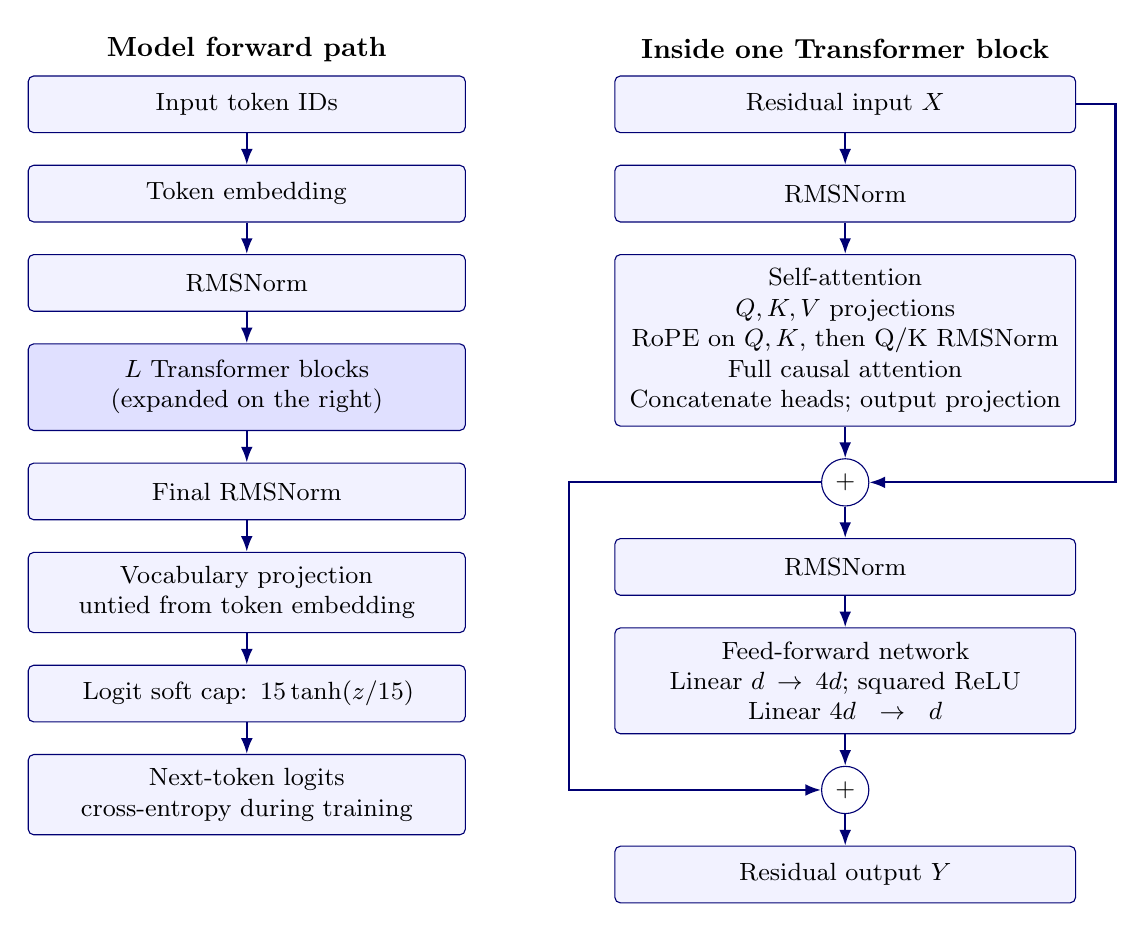
\begin{tikzpicture}[
 font=\small,
 box/.style={draw=blue!45!black,fill=blue!5,rounded corners=2pt,
 align=center,text width=5.2cm,minimum height=0.72cm,inner sep=5pt},
 detail/.style={box,text width=5.5cm},
 add/.style={circle,draw=blue!45!black,fill=white,inner sep=1pt,minimum size=6mm},
 flow/.style={-{Latex[length=2mm]},thick,draw=blue!45!black}]
 \node[font=\bfseries] at (0,0.7) {Model forward path};
 \node[font=\bfseries] at (7.6,0.7) {Inside one Transformer block};
 \node[box] (tokens) at (0,0) {Input token IDs};
 \node[box,below=4mm of tokens] (embed) {Token embedding};
 \node[box,below=4mm of embed] (initial) {RMSNorm};
 \node[box,below=4mm of initial,minimum height=1.1cm,fill=blue!12]
 (stack) {$L$ Transformer blocks\\(expanded on the right)};
 \node[box,below=4mm of stack] (final) {Final RMSNorm};
 \node[box,below=4mm of final] (head) {Vocabulary projection\\untied from token embedding};
 \node[box,below=4mm of head] (cap) {Logit soft cap: $15\tanh(z/15)$};
 \node[box,below=4mm of cap] (out) {Next-token logits\\cross-entropy during training};
 \foreach \a/\b in {tokens/embed,embed/initial,initial/stack,stack/final,final/head,head/cap,cap/out}
 \draw[flow] (\a) -- (\b);
 \node[detail] (input) at (7.6,0) {Residual input $X$};
 \node[detail,below=4mm of input] (norm1) {RMSNorm};
 \node[detail,below=4mm of norm1,minimum height=2cm] (attn)
 {Self-attention\\$Q,K,V$ projections\\RoPE on $Q,K$, then Q/K RMSNorm\\Full causal attention\\Concatenate heads; output projection};
 \node[add,below=4mm of attn] (add1) {$+$};
 \node[detail,below=4mm of add1] (norm2) {RMSNorm};
 \node[detail,below=4mm of norm2,minimum height=1.2cm] (mlp)
 {Feed-forward network\\Linear $d\to4d$; squared ReLU\\Linear $4d\to d$};
 \node[add,below=4mm of mlp] (add2) {$+$};
 \node[detail,below=4mm of add2] (output) {Residual output $Y$};
 \foreach \a/\b in {input/norm1,norm1/attn,attn/add1,add1/norm2,norm2/mlp,mlp/add2,add2/output}
 \draw[flow] (\a) -- (\b);
 \draw[flow] (input.east) -- ++(0.5,0) |- (add1.east);
 \draw[flow] (add1.west) -- ++(-3.2,0) |- (add2.west);
 \end{tikzpicture}%
 }
 \caption{Original nanochat architecture (October 13, 2025,
 commit \texttt{3a5e0bc}). Left: the complete forward path. Right: one
 pre-normalized Transformer block, repeated $L$ times. The two bypass
 arrows are residual connections. RoPE and Q/K normalization apply only
 to queries and keys, not values. All RMSNorm operations are parameter-free,
 and all linear projections are bias-free. Based on the original source
 code~\cite{nanochat-code}.}
 \label{fig:original}
\end{figure}

\clearpage
\subsection{From the original architecture to the July baseline}
The original diagram is historical context, not the model used for the
ablations. Comparing the October commit with the July 3 commit reveals the
following structural differences~\cite{nanochat-code,nanochat-july}.
\begin{table}[htbp]
\centering
\small
\begin{tabularx}{\linewidth}{@{}p{2.4cm}XX@{}}
\hline
Component & October 2025 & July 2026 baseline\\
\hline
Attention span & Full causal attention in each layer.
& SSSL sliding/full-window schedule; final layer uses the full context.\\
Value pathway & Each layer projects its own values from the residual stream.
& Still has per-layer K/V projections; adds gated token-value embeddings
in alternating layers, including the final layer.\\
Residual pathway & Ordinary pre-normalized residual additions.
& Adds learned residual scaling and initial-embedding blending, token
smearing, and subtraction of a cached intermediate residual (backout).\\
Position and heads & RoPE, Q/K RMSNorm, and GQA support.
& Retains these features; also scales normalized Q and K by 1.2 each.\\
\hline
\end{tabularx}
\caption{Selected code-level version differences. Gated value embeddings
are not FoX forget gates; GQA is not cross-layer K/V sharing; ordinary RoPE
is not FoPE.}
\end{table}
The July features remain common to the baseline and selected adaptations
unless explicitly changed below. Thus, our BPB differences compare
adaptations of the July model, not October versus July improvements.

\subsection{Three selected architecture proposals}
We select Forgetting Transformer (FoX), Cross-Layer Attention (CLA), and
Fourier Position Embedding (FoPE) as the three literature-backed proposals
for Part One. Their source papers appeared at ICLR 2025, NeurIPS 2024,
and ICML 2025, respectively~\cite{fox,cla,fope}. Publication supports their
use as research sources; it does not guarantee improvements in nanochat.
Table~\ref{tab:proposals} distinguishes their motivations, mechanisms,
and hypothesized effects. The hypotheses are not measured results.

\begin{table}[htbp]
\centering
\footnotesize
\renewcommand{\arraystretch}{1.15}
\begin{tabularx}{\linewidth}{@{}p{1.7cm}XXX@{}}
\hline
Change & Motivation & Technical change & Measurable hypothesis\\
\hline
FoX~\cite{fox} & Allow attention to forget irrelevant history in an
input-dependent way. & Add cumulative log-sigmoid forget gates to causal
attention logits, down-weighting older keys according to intervening gates;
the proposed model does not require positional embeddings.
& At equal training tokens and on the same evaluation corpus, lower
validation BPB than baseline at context 512. Extrapolation is a separate,
currently untested hypothesis.\\
\hline
CLA~\cite{cla} & Reduce the memory required for the autoregressive KV cache.
& Reuse projected keys and values across adjacent layers, while queries
remain layer-specific. CLA2 shares across pairs of layers.
& Quality: sharing increases BPB relative to baseline. Memory: a shared-cache
implementation reduces inference KV bytes at fixed batch/context/dtype.
Only the quality hypothesis is tested here.\\
\hline
FoPE~\cite{fope} & Improve positional representations outside the training
context length. & Replace individual rotary-frequency components with
Fourier-series representations and remove inadequately trained low-frequency
components. & After equal training at context 512, lower BPB than RoPE
at context 2048 on identical held-out tokens, without further training.
Proposed only; not tested in Part Two.\\
\hline
\end{tabularx}
\caption{The three selected proposals. These are different interventions:
attention forgetting, cross-layer sharing, and positional representation.}
\label{tab:proposals}
\end{table}

\paragraph{Operational definitions and decision rules.}
For each paired seed $s$, define
$\Delta_s=\mathrm{BPB}_{\mathrm{variant},s}-\mathrm{BPB}_{\mathrm{baseline},s}$
on the same held-out tokens at context 512 and after 16,384,000 training
tokens. For FoX, the directional quality hypothesis is $\Delta_s<0$;
we report each seed and their mean rather than treating two seeds as a
significance test. For CLA2, the directional quality-cost hypothesis is
$\Delta_s>0$: sharing may reduce representational capacity. We quantify
the degradation rather than calling it negligible without a predefined
acceptable BPB margin. These are exploratory interpretations formulated
for this report after screening, not preregistered hypotheses.

The distinct CLA memory hypothesis is
$M_{\mathrm{KV,CLA2}}<M_{\mathrm{KV,baseline}}$, where $M_{\mathrm{KV}}$
counts stored inference K/V tensor bytes at equal batch size, context length,
head dimensions, and dtype. Total training peak VRAM and parameter count
are not substitutes for this measurement. An ideal pair-shared cache stores
half as many layer-specific K/V tensors, but our recipient-specific value
embeddings complicate sharing the final values; we neither implement that
cache nor claim a measured twofold saving.

FoPE's proposed length test compares models trained at 512 and evaluated
without updates at 512, 1024, and 2048 on a common set of target tokens,
changing only the available preceding context. The primary proposed
contrast is BPB at 2048, with in-range BPB reported separately. Continued
training at 2048 would instead test context adaptation, not zero-shot
extrapolation. Likewise, FoX's positive 512-token result cannot establish
long-context generalization.

\paragraph{Selection for Part Two.}
We select \textbf{FoX and CLA2} for the two individual architecture
ablations, each compared against the same baseline. FoX tests a quality
hypothesis; the current CLA2 experiment tests the quality side of an
efficiency--quality trade-off, not its inference-memory benefit. FoPE remains our
third literature proposal, not a selected Part Two ablation. A negative CLA2 quality result is
informative, but training throughput alone cannot validate the paper's
inference-cache claim. No combined FoX--CLA2 model has been tested.

\paragraph{Scope and implementation fidelity.}
Our implementation details below describe adaptations, not exact paper
reproductions. In particular, CLA2 is not FusedKV-Lite; the current code
does not implement shared inference caching. Inspection of the July baseline
confirms that it does not implement FoX-style cumulative forgetting,
cross-layer K/V sharing, or FoPE. Its value-embedding gates, per-layer K/V
projections and caches, and ordinary RoPE are distinct from these proposals.
We do not claim these ideas have never
been attempted in another nanochat fork.

\clearpage
\section{Part Two: Picochat Ablations}
\subsection{Purpose and protocol}
We compare the two selected adaptations, FoX and CLA2, individually against
an unmodified pilot baseline. These are short exploratory ablations, not
full paper reproductions or a final-model evaluation. The six primary runs
completed on November 3, 2026: three configurations with seeds 42 and 43.
Two subsequent runs on the same date retain RoPE in FoX as a mechanism
control, not a third selected architecture change.
Each run used 500 optimizer steps of 32,768 tokens,
or 16,384,000 training tokens, with 262,144 held-out validation tokens.
Validation bits per byte (BPB) is the primary metric; lower is better.

The pilot used nanochat commit
\texttt{92d63d4e8bb4df75c3b71618f31ddde2378b2bcd}, six layers,
width 384, six attention heads, a 512-token context, and the SSSL window
schedule. A 32,768-token BPE tokenizer was trained on 100M characters
from four ClimbMix training shards. Runs used a separate validation shard,
common-parameter initialization seeds and the same deterministic data order,
upstream Muon/AdamW parameter grouping, a common learning-rate schedule,
and BF16 on an NVIDIA H100 80GB HBM3 GPU.
Model execution was eager; optimizer kernels were compiled.
CUDA deterministic algorithms were not forced.

\subsection{Implemented adaptations}
\begin{description}
\item[Cross-layer sharing (CLA2)~\cite{cla}.] Adjacent layers share projected keys and
values, retaining recipient-specific value embeddings and removing receiver
K/V projections. This is a CLA adaptation, not FusedKV-Lite. No shared
inference cache was implemented or benchmarked.
Sharing is applied to raw projected K/V before RoPE and before adding
each recipient's own value embedding. This preserves a July-baseline
feature but differs from simply reusing identical final K/V tensors across
layers. Accordingly, the result evaluates this specific adaptation, not
the paper's complete inference design.
\item[Forgetting Transformer (FoX)~\cite{fox}.] Accumulated log-sigmoid forget gates
modify attention logits; RoPE is removed. Nanochat Q/K normalization and
value embeddings are retained. This uses dense reference attention, not
the paper's optimized kernel.
The ablation changes both the attention scores and the positional treatment
(removing RoPE). It therefore measures their joint effect, not the isolated
causal contribution of the forget gate. The follow-up below adds a gates-with-RoPE
control; a no-gates/no-RoPE control remains missing. The July window
schedule, residual pathways, and value embeddings remain in place.
\end{description}

\subsection{Selected Part Two ablations: preliminary results}
Table~\ref{tab:selected-ablations} compares the two selected changes with
the baseline. All values are from the existing short pilot; this
selection did not involve additional training. The baseline has approximately
73.5M parameters. Its small depth, width, and 512-token context make repeated
controlled comparisons inexpensive, but also limit conclusions about larger
models and longer contexts.
\begin{table}[htbp]
\centering
\small
\begin{tabular}{lrrrr}
\hline
Configuration & Seed 42 BPB & Seed 43 BPB & Mean BPB & Difference\\
\hline
Baseline & 1.36560 & 1.35770 & 1.36165 & $0.00000$\\
Baseline + FoX & 1.35234 & 1.34357 & 1.34795 & $-0.01370$\\
Baseline + CLA2 & 1.39346 & 1.38805 & 1.39075 & $+0.02910$\\
\hline
\end{tabular}
\caption{Selected individual ablations; lower BPB is better. FoX improves
both seeds, whereas CLA2 worsens both. Differences are relative to the
baseline mean. These are not results for a combined model.}
\label{tab:selected-ablations}
\end{table}

\subsection{Follow-up control: forgetting gates with RoPE}
We trained the FoX adaptation with RoPE retained for the same two seeds,
500 steps, and 16.384M tokens per run. Model configuration, optimizer,
data order, and evaluation protocol were unchanged. Both runs completed.
CPU and GPU checks verified identical initial parameters between the two
FoX variants and that identity rotations recover the original FoX outputs.
A source-hash audit confirmed that the original variant code was unchanged
apart from adding the new branch.
\begin{table}[htbp]
\centering
\small
\begin{tabular}{lrrrr}
\hline
Configuration & Seed 42 BPB & Seed 43 BPB & Mean BPB & Tokens/s\\
\hline
Baseline (RoPE, no gates) & 1.36560 & 1.35770 & 1.36165 & 233,814\\
FoX (gates, no RoPE) & 1.35234 & 1.34357 & 1.34795 & 209,240\\
FoX (gates + RoPE) & 1.34756 & 1.34840 & 1.34798 & 176,929\\
\hline
\end{tabular}
\caption{Fixed-token RoPE control. Baseline and no-RoPE FoX are the earlier
pilot runs; the new runs are not concurrent timing controls.}
\end{table}
With RoPE retained, forgetting attention improves BPB over baseline in both
seeds (differences $-0.01804$ and $-0.00930$). Its mean is nearly identical
to no-RoPE FoX: a difference of approximately $+0.00003$ BPB, with opposite
directions across seeds. Thus, removing RoPE is not necessary to obtain a
fixed-token improvement in these runs. This is not proof that the two FoX
variants are equivalent, nor evidence of long-context generalization.

The new mean throughput is about 24.3\% below the historical baseline and
15.4\% below historical no-RoPE FoX. These are observed cross-run differences,
not an isolated measurement of RoPE overhead: the new seeds themselves
achieved 184,462 and 169,396 tokens/s. Hardware/runtime variability and the
dense reference kernel limit causal timing conclusions. A concurrent,
repeated microbenchmark would be needed to isolate RoPE's runtime cost.

\subsection{Training efficiency}
\begin{table}[htbp]
\centering
\small
\begin{tabular}{lrrrr}
\hline
Variant & Parameters & Tokens/s & Throughput change & Peak GiB\\
\hline
Baseline & 73,531,646 & 233,814 & --- & 3.16\\
CLA2 & 72,646,910 & 238,817 & $+2.1\%$ & 3.15\\
FoX & 73,545,506 & 209,240 & $-10.5\%$ & 3.64\\
\hline
\end{tabular}
\caption{Mean steady training throughput across seeds and maximum peak
allocated GPU memory across seeds. These are implementation-specific
training measurements, not inference-cache benchmarks.}
\end{table}

\paragraph{Equal tokens versus equal training budget.}
FoX improves mean BPB at equal training tokens but has 10.5\% lower measured
throughput. CLA2 is 2.1\% faster but has worse BPB. Neither result establishes
which model achieves the lowest BPB within a fixed GPU-time budget.
Using the mean steady-state rates as an approximation,
$233{,}814/209{,}240\approx1.117$: the baseline could process about 11.7\%
more tokens in the time FoX processes a fixed token budget. Thus, in the
steady training time needed for FoX's 16.384M tokens, the baseline could
potentially process approximately 18.31M tokens. Equivalently, FoX takes
about 11.7\% longer for equal tokens; this is not the same percentage as
its 10.5\% throughput reduction.

These calculations assume stable throughput and exclude differences in
startup, evaluation, and compilation overhead. They are budget projections,
not measured BPB results at 18.31M tokens. Additional baseline training
might narrow, eliminate, or reverse FoX's advantage, but our data do not
establish which outcome occurs. The small CLA2 throughput difference also
needs repeated timing measurements before being treated as a robust speedup.

A follow-up should compare validation BPB against cumulative training GPU
seconds, or total billed cost, using identical hardware and reporting
setup/evaluation overhead separately. Each run's learning-rate schedule
should be specified for its intended training horizon, rather than extending
an already annealed baseline arbitrarily. Equal GPU time on one GPU type
approximates equal GPU cost, but is not equal mathematical FLOPs: kernel
efficiency and architectural work differ. Our dense FoX reference attention
also makes the measured slowdown implementation-specific; it is not a
benchmark of the paper's optimized kernel. We therefore nominate FoX as
the better \emph{fixed-token quality} candidate, not a demonstrated
fixed-compute or fixed-cost winner. No additional budget-matched experiment
has been conducted.

\subsection{Interpretation and limitations}
FoX is the stronger fixed-token quality candidate for a longer follow-up: it improved BPB in
both paired seeds, with an approximately 1.0\% reduction in mean BPB.
Its paired BPB differences are $-0.01326$ and $-0.01414$, consistent with
the directional short-context quality hypothesis in this pilot only.
Here ``FoX improves BPB'' refers specifically to the combined adaptation:
forgetting gates plus removal of RoPE. It does not establish that the gates
alone cause the improvement; removing RoPE or an interaction between the
two changes could contribute.
CLA2 worsened BPB in both seeds, while using fewer parameters and slightly
higher measured training throughput. We have not measured its potential
shared-cache inference benefit. Neither result guarantees the same outcome
under longer training, larger models, or other evaluation settings.
CLA2's paired differences are $+0.02786$ and $+0.03035$ (mean $+0.02910$);
this supports a quality-cost observation, not a demonstrated beneficial
memory--quality trade-off. The separate cache-memory hypothesis remains
untested.

\paragraph{Confounding changes and missing controls.}
The baseline provides RoPE without forgetting; the new control adds
forgetting with RoPE held fixed. This strengthens evidence that the
forgetting-attention adaptation can help without changing positional
representation. It is not a perfectly isolated gate comparison because
the reference attention implementation and a small number of additional
parameters also differ from baseline. A full four-condition comparison
still requires baseline attention without RoPE, which has not been run.
Without that cell, the RoPE-removal effect without gates and the full
interaction between gates and positional representation remain unidentified.

CLA2 has 72,646,910 parameters versus the baseline's 73,531,646: 884,736
fewer parameters (approximately 1.20\%). Its worse BPB could reflect reduced
representational capacity from sharing K/V projections, not an inherently
ineffective architectural idea. The current experiment cannot separate
parameter reduction from the sharing constraint. A follow-up could compare
CLA2 with a parameter-budget-matched unshared baseline and, separately,
reallocate the saved parameters in CLA2 to test the quality at a common
budget. Such controls would still change parameter allocation and would
not automatically match FLOPs or wall-clock cost. We have not run them.

Thus, the fixed-token results do not establish parameter-efficiency or
compute-efficiency superiority: this comparison is neither parameter-matched
nor FLOP-matched. It uses only
two seeds and a short training horizon. It does not test context extension,
cached decoding, CORE, SFT, or conversational quality.
Architecture adaptations and reference kernels also limit comparisons to
published paper results. Final-model decisions require longer runs rather
than extrapolating directly from these short pilot results.

\paragraph{Implications for a larger nanochat run.}
Table~\ref{tab:scaling-hypotheses} states our explicit expectations and the
uncertainties that a larger run would need to resolve. These are hypotheses,
not extrapolated measurements or fitted scaling laws.
\begin{table}[htbp]
\centering
\small
\begin{tabularx}{\linewidth}{@{}p{1.2cm}XX@{}}
\hline
Change & Larger-run hypothesis & Important uncertainty\\
\hline
FoX & The lower BPB observed at equal tokens may persist at larger model
sizes if learned forgetting remains useful.
& Added attention work and our dense implementation could become expensive,
especially at longer contexts. The quality benefit may not survive an
equal-time comparison; optimized kernels could change the trade-off.\\
CLA2 & Shared-cache memory savings may matter more during long-context,
large-batch inference, potentially permitting a larger serving workload.
& The quality penalty may persist or change with model size. Our
recipient-specific value embeddings require a suitable cache design, and
the current implementation has not demonstrated inference savings.\\
\hline
\end{tabularx}
\caption{Larger-run expectations for the two selected interventions.}
\label{tab:scaling-hypotheses}
\end{table}

CLA2's quality penalty may persist, shrink, or grow with model size and
training duration. Larger models might compensate for shared projections
using capacity elsewhere, or sharing might remain a bottleneck; neither
possibility is established by our single-scale pilot. Conversely, a correctly
implemented shared cache could become more useful as layer count, batch
size, and context length increase, even if a quality penalty remains.
Our current implementation does not measure that benefit. The decision
to use CLA2 at scale should therefore depend on an empirically measured
quality--memory trade-off, not BPB or parameter count alone.

Similarly, FoX's short-run BPB advantage could persist, disappear, or reverse
after longer training or at larger scale. It does not by itself predict
better long-context retrieval or conversational performance. A stronger
scaling study would repeat the matched-token comparisons at multiple model
sizes, report paired BPB differences and training costs, and separately
measure inference cache bytes and long-context evaluation. Equal-token
comparisons should be distinguished from equal-compute comparisons because
the interventions change parameter counts and computational work.

\subsection{Execution, cost, and reproducibility}
CPU and GPU smoke tests checked finite forward/backward computation,
gradient presence, causal prefix invariance, checkpoint loading, and baseline
agreement with upstream nanochat. A local metadata-deserialization failure
interrupted some initial attempts. Completed results were preserved; only
missing runs were restarted after fixing metadata serialization. Interrupted
attempts are excluded from the tables and remain visible in W\&B.

For the six reported baseline/FoX/CLA2 runs, successful seed-function
elapsed time totalled 563.0 seconds, corresponding to an estimated \$0.62
of GPU time at \$0.001097 per second. The broader exploratory campaign
used an estimated \$1.75 of successful-run GPU time, including experiments
outside this report's selected ablations. The later RoPE-control runs add
219.5 seconds of successful seed-function time, approximately \$0.24 of
GPU time, bringing the successful-run campaign estimate to about \$1.99.
None of these figures represents
\emph{the total bill}: startup, preparation, smoke tests, interrupted
attempts, and CPU/RAM add cost. The final invoice has not been verified.
The approved pilot ceiling was \$40. No further training was launched
after collection; the Modal app listing was empty at that check.

Raw results are stored in \texttt{a3/pilot\_results/sweep.json}; the
companion report retains the complete exploratory record and run links.
The results reported here select only baseline, FoX, and CLA2, seeds 42 and 43.
The additional FoX control is saved separately in
\texttt{a3/pilot\_results/rope-control.json}; its summary and individual
W\&B links are in \texttt{a3/pilot\_results/ROPE\_CONTROL.md}.
The experiment dashboard is
\href{https://wandb.ai/jinhaozhang123-university-of-toronto/a3-picochat-pilot}{the W\&B picochat pilot project}.

\paragraph{Draft status.}
This is an architecture review and exploratory pilot report, not a finished
assignment submission. Required context-extension/final-model experiments, team details,
and final layout review remain to be completed.
\clearpage
\begin{thebibliography}{99}
\bibitem{nanochat-readme}
Andrej Karpathy. \emph{Nanochat: The best ChatGPT that \$100 can buy}.
Repository README, original October 13, 2025 snapshot.
\url{https://github.com/karpathy/nanochat/blob/3a5e0bc50b123f37220f1ace6813f080455d19f3/README.md}.

\bibitem{nanochat-code}
Andrej Karpathy. \emph{Nanochat model implementation: nanochat/gpt.py}.
Commit \texttt{3a5e0bc50b123f37220f1ace6813f080455d19f3}, October 13, 2025.
\url{https://github.com/karpathy/nanochat/blob/3a5e0bc50b123f37220f1ace6813f080455d19f3/nanochat/gpt.py}.

\bibitem{nanochat-july}
Andrej Karpathy. \emph{Nanochat model implementation: nanochat/gpt.py}.
Commit \texttt{92d63d4e8bb4df75c3b71618f31ddde2378b2bcd}, July 3, 2026.
\url{https://github.com/karpathy/nanochat/blob/92d63d4e8bb4df75c3b71618f31ddde2378b2bcd/nanochat/gpt.py}.

\bibitem{fox}
Zhixuan Lin, Evgenii Nikishin, Xu Owen He, and Aaron Courville.
\emph{Forgetting Transformer: Softmax Attention with a Forget Gate}.
International Conference on Learning Representations (ICLR), 2025.
\url{https://openreview.net/forum?id=q2Lnyegkr8}.

\bibitem{cla}
William Brandon, Mayank Mishra, Aniruddha Nrusimha, Rameswar Panda,
and Jonathan Ragan-Kelley.
\emph{Reducing Transformer Key-Value Cache Size with Cross-Layer Attention}.
Advances in Neural Information Processing Systems (NeurIPS), 2024.
\url{https://arxiv.org/abs/2405.12981}.

\bibitem{fope}
Ermo Hua, Che Jiang, Xingtai Lv, Kaiyan Zhang, Youbang Sun, Yuchen Fan,
Xuekai Zhu, Biqing Qi, Ning Ding, and Bowen Zhou.
\emph{Fourier Position Embedding: Enhancing Attention's Periodic Extension
for Length Generalization}.
Proceedings of the 42nd International Conference on Machine Learning,
PMLR 267:24932--24949, 2025.
\url{https://proceedings.mlr.press/v267/hua25b.html}.
\end{thebibliography}
\end{document}
